% Gemini theme
% https://github.com/anishathalye/gemini

\documentclass[final]{beamer}

% ====================
% Color options
% ====================

\newif\ifgrayhighlight % define new flag
% \grayhighlighttrue     % Use gray background for highlighted block
\grayhighlightfalse    % Use cardinal red background for highlighted block

% ====================
% Packages
% ====================

\usepackage[T1]{fontenc}
\usepackage{lmodern}
\usepackage[size=custom,width=120,height=120,scale=1.0]{beamerposter}
\usetheme{gemini}
\usecolortheme{stanford}
\usepackage{graphicx}
\usepackage{booktabs}
\usepackage{tikz}
\usepackage{pgfplots}
\pgfplotsset{compat=1.14}
\usepackage{anyfontsize}

% ====================
% Lengths
% ====================

% If you have N columns, choose \sepwidth and \colwidth such that
% (N+1)*\sepwidth + N*\colwidth = \paperwidth
\newlength{\sepwidth}
\newlength{\colwidth}
\setlength{\sepwidth}{0.025\paperwidth}
\setlength{\colwidth}{0.3\paperwidth}

\newcommand{\separatorcolumn}{\begin{column}{\sepwidth}\end{column}}

% ====================
% Title
% ====================

\title{Software Best Practices for Reproducible Open Science}

\author{Alex Koufos \inst{1}} %\and Ben Bitdiddle \inst{1}}

\institute[shortinst]{\inst{1} Stanford University}

% ====================
% Footer (optional)
% ====================

\footercontent{
  \href{https://github.com/exoticdft}{https://github.com/exoticdft} \hfill
  TESS/SPD 2024 - Dallas, TX --- 211-040 \hfill
  \href{mailto:akoufos@sun.stanford.edu}{akoufos@sun.stanford.edu}
}
% (can be left out to remove footer)

% ====================
% Logo (optional)
% ====================

% use this to include logos on the left and/or right side of the header:
\logoleft{
\includegraphics[height=3cm]{logos/stanford+solar_group+HEPL-white.pdf}}
\logoright{
\includegraphics[height=7cm]{logos/SUTree-2color.pdf}}

% ====================
% Body
% ====================

\begin{document}

\begin{frame}[t]
\begin{columns}[t]
\separatorcolumn

\begin{column}{\colwidth}

  \begin{block}{Is there a "reproducibility crisis" in the sciences?}

    Over the past two decades, many researchers have been discussing the
    potential issue within the whole of the science communities related to the
    ability to reproduce the scientific work of others, and even themselves.
    This issue has been termed the "Reproducibility Crisis" in the sciences.
    A recent Nature article\cite{baker2016} discusses this issue.
       
    \begin{figure}
      \centering
      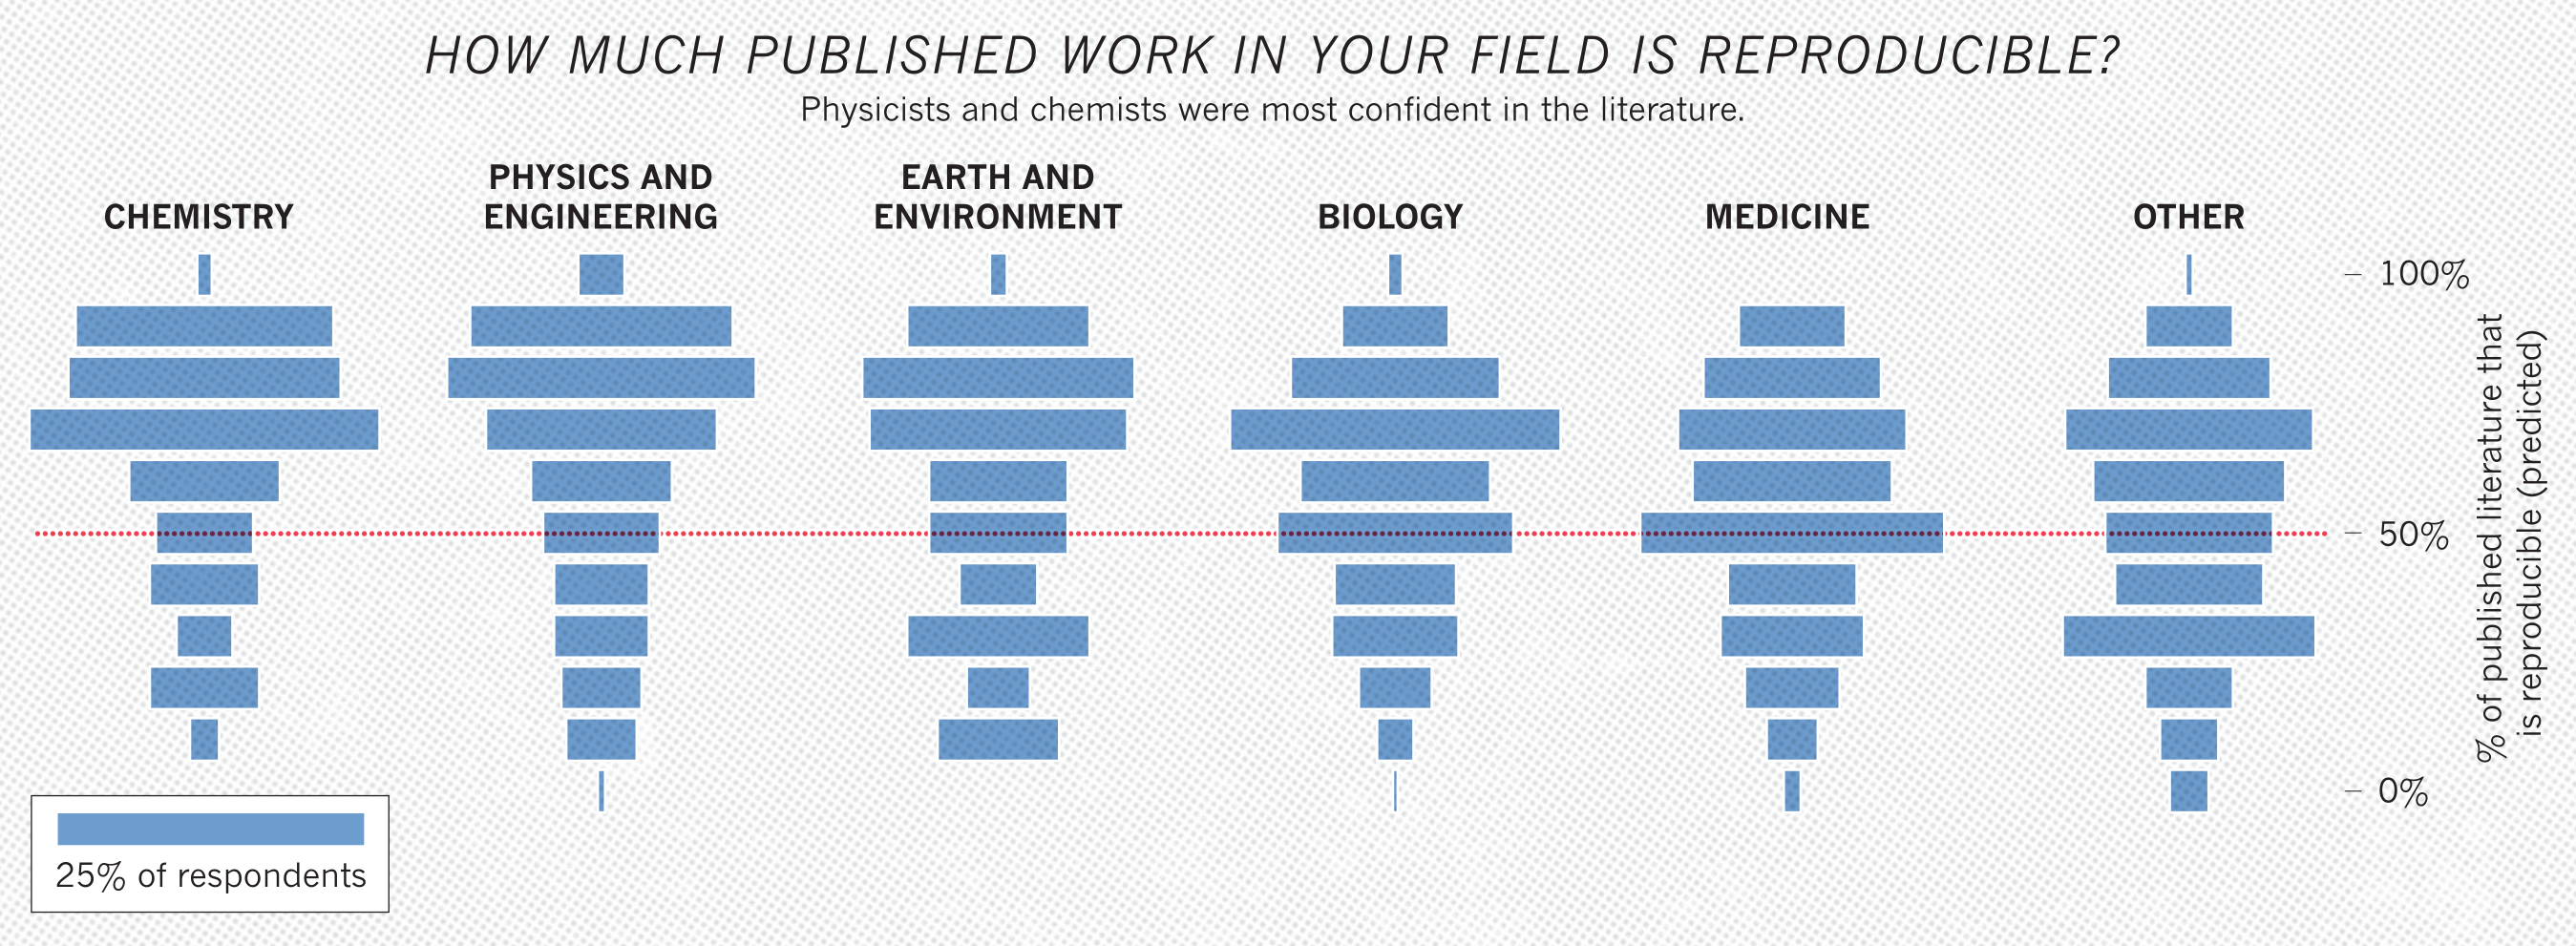
\includegraphics[width=0.85\textwidth]{tess2024/Nature-Field-Confidence.png}
      \caption{Science Field Based Confidence in Published Work (Baker, M. 2016)}
      \label{fig:confidence}
    \end{figure}

    Figure \ref*{fig:confidence} shows the general concern from those in the
    scientific community.
    In general, the physics and engineering community tends to be more
    confident in published literature.
    However, the research suggest there are still many researchers who are not
    confident.
    This issue leads to a lack of confidence from the general public.

    \begin{figure}
      \centering
      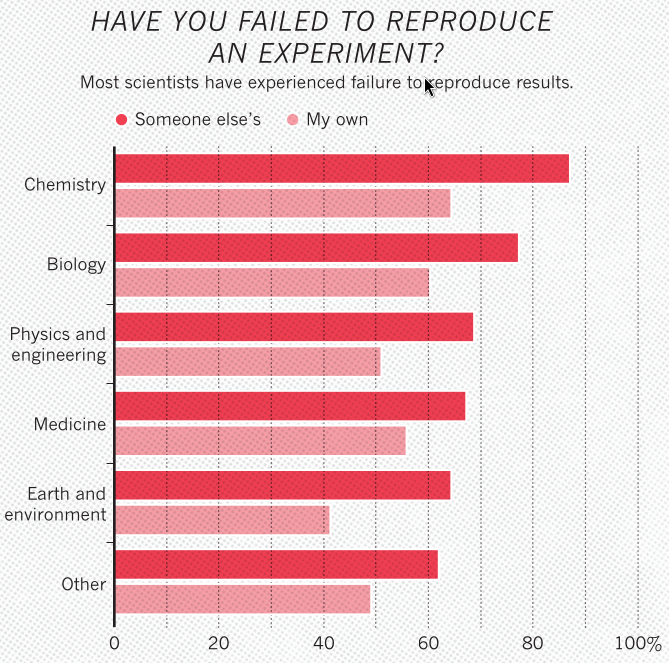
\includegraphics[width=0.85\textwidth]{tess2024/Nature-Reproducibility-Failure-.png}
      \caption{Failure to Reproduce Published Results (Baker, M. 2016)}
      \label{fig:failure}
    \end{figure}
    
    Figure \ref*{fig:failure} provides another metric for understanding this
    crisis.
    In all research communities, many researchers struggled to reproduce the
    results of others, and even themselves.
    This included the physics and engineering communities.

  \end{block}

  \begin{alertblock}{A Failure to Reproduce}
    Several reports have suggested there is a problem with researchers being
    able to reproduce their own work.
    The numbers suggest \textbf{over 50\% of the physics and engineering community
    were unable to reproduce their own work!}

  \end{alertblock}

  \begin{block}{But what is Reproducibility?}
    In 2019, a National Academy of Sciences committee exploring the
    reproducibility and replicability in scientific and engineering research.
    The committee define\cite{reproducibility_in_science}
    \begin{description}
      \item[reproducibility (i.e. computational reproducibility)] \hfill \\
      as obtaining consistent computational results using the same input data,
      computational steps, methods, code, and conditions of analysis
      \item[replicability] \hfill \\
      as obtaining consistent results across studies aimed at answering the same
      scientific question, each of which has obtained its own data
    \end{description}

    This poster will focus on the former definition.
    There are many techniques we can all use to help alleviate potential issues
    with being able to reproduce results.

  \end{block}

\end{column}

\separatorcolumn

\begin{column}{\colwidth}

  \begin{block}{Ways to help mitigate the reproducibility in your research}

    Today, computers are used in ever aspect of research.
    Although software is inherit in our research to do simple or complex
    computations, we don't always look at these efforts as software engineering.
    However, we can learn a lot from the community and in the recent years
    some associations have come about focused on "research software engineering"
    (RSEng).
    One such is the 
    (\href{https://us-rse.org}{United States Research Software Engineer Association (US-RSE)})
    (several others are mentioned in the references section.)
    These communities strive to promote scientific best practices for better
    research related software.
    For example, the Better Scientific Software (BSSw)\cite{bssw} provides many
    resources to help researchers and RSEs support successful research projects.

    Although these resources can be extremely useful, their are some many
    "best practices" out there to investigate.
    So I'm going to discuss some of the "easier" and possibly most impactful
    tools one can use.
    
    \textbf{Disclaimer:} None of the these techniques can single handedly
    resolve, or entirely mitigate the problem of reproducibility.
    However, together they can help reduce unintended difficulties for others,
    or even yourself, in reproducing your work in the future.

    \begin{enumerate}
      \item \textbf{Version Control} 
      \item \textbf{Code Reviews} 
      \item \textbf{Documentation} 
      \item \textbf{Testing} 
    \end{enumerate}

  \end{block}

  \begin{block}{Version Control}

    

    \begin{figure}
      \centering
      \begin{tikzpicture}
        \begin{axis}[
            scale only axis,
            no markers,
            domain=0:2*pi,
            samples=100,
            axis lines=center,
            axis line style={-},
            ticks=none]
          \addplot[red] {sin(deg(x))};
          \addplot[blue] {cos(deg(x))};
        \end{axis}
      \end{tikzpicture}
      \caption{Another figure caption.}
    \end{figure}

  \end{block}

  \begin{block}{Documentation}

    Nulla eget sem quam. Ut aliquam volutpat nisi vestibulum convallis. Nunc a
    lectus et eros facilisis hendrerit eu non urna. Interdum et malesuada fames
    ac ante \textit{ipsum primis} in faucibus. Etiam sit amet velit eget sem
    euismod tristique. Praesent enim erat, porta vel mattis sed, pharetra sed
    ipsum. Morbi commodo condimentum massa, \textit{tempus venenatis} massa
    hendrerit quis. Maecenas sed porta est. Praesent mollis interdum lectus,
    sit amet sollicitudin risus tincidunt non.

    Etiam sit amet tempus lorem, aliquet condimentum velit. Donec et nibh
    consequat, sagittis ex eget, dictum orci. Etiam quis semper ante. Ut eu
    mauris purus. Proin nec consectetur ligula. Mauris pretium molestie
    ullamcorper. Integer nisi neque, aliquet et odio non, sagittis porta justo.

    \begin{itemize}
      \item \textbf{Sed consequat} id ante vel efficitur. Praesent congue massa
        sed est scelerisque, elementum mollis augue iaculis.
        \begin{itemize}
          \item In sed est finibus, vulputate
            nunc gravida, pulvinar lorem. In maximus nunc dolor, sed auctor eros
            porttitor quis.
          \item Fusce ornare dignissim nisi. Nam sit amet risus vel lacus
            tempor tincidunt eu a arcu.
          \item Donec rhoncus vestibulum erat, quis aliquam leo
            gravida egestas.
        \end{itemize}
      \item \textbf{Sed luctus, elit sit amet} dictum maximus, diam dolor
        faucibus purus, sed lobortis justo erat id turpis.
      \item \textbf{Pellentesque facilisis dolor in leo} bibendum congue.
        Maecenas congue finibus justo, vitae eleifend urna facilisis at.
    \end{itemize}

  \end{block}

\end{column}

\separatorcolumn

\begin{column}{\colwidth}

  \begin{exampleblock}{A highlighted block containing some math}

    A different kind of highlighted block.

    $$
    \int_{-\infty}^{\infty} e^{-x^2}\,dx = \sqrt{\pi}
    $$

    Interdum et malesuada fames $\{1, 4, 9, \ldots\}$ ac ante ipsum primis in
    faucibus. Cras eleifend dolor eu nulla suscipit suscipit. Sed lobortis non
    felis id vulputate.

    \heading{A heading inside a block}

    Praesent consectetur mi $x^2 + y^2$ metus, nec vestibulum justo viverra
    nec. Proin eget nulla pretium, egestas magna aliquam, mollis neque. Vivamus
    dictum $\mathbf{u}^\intercal\mathbf{v}$ sagittis odio, vel porta erat
    congue sed. Maecenas ut dolor quis arcu auctor porttitor.

    \heading{Another heading inside a block}

    Sed augue erat, scelerisque a purus ultricies, placerat porttitor neque.
    Donec $P(y \mid x)$ fermentum consectetur $\nabla_x P(y \mid x)$ sapien
    sagittis egestas. Duis eget leo euismod nunc viverra imperdiet nec id
    justo.

  \end{exampleblock}

  \begin{block}{Code Reviews}

    Class aptent taciti sociosqu ad litora torquent per conubia nostra, per
    inceptos himenaeos. Phasellus libero enim, gravida sed erat sit amet,
    scelerisque congue diam. Fusce dapibus dui ut augue pulvinar iaculis.

    \begin{table}
      \centering
      \begin{tabular}{l r r c}
        \toprule
        \textbf{First column} & \textbf{Second column} & \textbf{Third column} & \textbf{Fourth} \\
        \midrule
        Foo & 13.37 & 384,394 & $\alpha$ \\
        Bar & 2.17 & 1,392 & $\beta$ \\
        Baz & 3.14 & 83,742 & $\delta$ \\
        Qux & 7.59 & 974 & $\gamma$ \\
        \bottomrule
      \end{tabular}
      \caption{A table caption.}
    \end{table}

    Donec quis posuere ligula. Nunc feugiat elit a mi malesuada consequat. Sed
    imperdiet augue ac nibh aliquet tristique. Aenean eu tortor vulputate,
    eleifend lorem in, dictum urna. Proin auctor ante in augue tincidunt
    tempor. Proin pellentesque vulputate odio, ac gravida nulla posuere
    efficitur. Aenean at velit vel dolor blandit molestie. Mauris laoreet
    commodo quam, non luctus nibh ullamcorper in. Class aptent taciti sociosqu
    ad litora torquent per conubia nostra, per inceptos himenaeos.

    Nulla varius finibus volutpat. Mauris molestie lorem tincidunt, iaculis
    libero at, gravida ante. Phasellus at felis eu neque suscipit suscipit.
    Integer ullamcorper, dui nec pretium ornare, urna dolor consequat libero,
    in feugiat elit lorem euismod lacus. Pellentesque sit amet dolor mollis,
    auctor urna non, tempus sem.

  \end{block}

  \begin{block}{Testing}

    Class aptent taciti sociosqu ad litora torquent per conubia nostra, per
    inceptos himenaeos. Phasellus libero enim, gravida sed erat sit amet,
    scelerisque congue diam. Fusce dapibus dui ut augue pulvinar iaculis.

    Donec quis posuere ligula. Nunc feugiat elit a mi malesuada consequat. Sed
    imperdiet augue ac nibh aliquet tristique. Aenean eu tortor vulputate,
    eleifend lorem in, dictum urna. Proin auctor ante in augue tincidunt
    tempor. Proin pellentesque vulputate odio, ac gravida nulla posuere
    efficitur. Aenean at velit vel dolor blandit molestie. Mauris laoreet
    commodo quam, non luctus nibh ullamcorper in. Class aptent taciti sociosqu
    ad litora torquent per conubia nostra, per inceptos himenaeos.

  \end{block}

  \begin{block}{References}

    \nocite{*}
    \footnotesize{\bibliographystyle{plain}\bibliography{poster}}

  \end{block}

\end{column}

\separatorcolumn
\end{columns}
\end{frame}

\end{document}
